%% BioMed_Central_Tex_Template_v1.06
%%                                      %
%  bmc_article.tex            ver: 1.06 %
%                                       %

%%IMPORTANT: do not delete the first line of this template
%%It must be present to enable the BMC Submission system to
%%recognise this template!!

%%%%%%%%%%%%%%%%%%%%%%%%%%%%%%%%%%%%%%%%%
%%                                     %%
%%  LaTeX template for BioMed Central  %%
%%     journal article submissions     %%
%%                                     %%
%%          <8 June 2012>              %%
%%                                     %%
%%                                     %%
%%%%%%%%%%%%%%%%%%%%%%%%%%%%%%%%%%%%%%%%%


%%%%%%%%%%%%%%%%%%%%%%%%%%%%%%%%%%%%%%%%%%%%%%%%%%%%%%%%%%%%%%%%%%%%%
%%                                                                 %%
%% For instructions on how to fill out this Tex template           %%
%% document please refer to Readme.html and the instructions for   %%
%% authors page on the biomed central website                      %%
%% http://www.biomedcentral.com/info/authors/                      %%
%%                                                                 %%
%% Please do not use \input{...} to include other tex files.       %%
%% Submit your LaTeX manuscript as one .tex document.              %%
%%                                                                 %%
%% All additional figures and files should be attached             %%
%% separately and not embedded in the \TeX\ document itself.       %%
%%                                                                 %%
%% BioMed Central currently use the MikTex distribution of         %%
%% TeX for Windows) of TeX and LaTeX.  This is available from      %%
%% http://www.miktex.org                                           %%
%%                                                                 %%
%%%%%%%%%%%%%%%%%%%%%%%%%%%%%%%%%%%%%%%%%%%%%%%%%%%%%%%%%%%%%%%%%%%%%

%%% additional documentclass options:
%  [doublespacing]
%  [linenumbers]   - put the line numbers on margins

%%% loading packages, author definitions

%\documentclass[twocolumn]{bmcart}% uncomment this for twocolumn layout and comment line below
\documentclass{bmcart}

%%% Load packages
%\usepackage{amsthm,amsmath}
\usepackage{amssymb}
%\RequirePackage{natbib}
%\RequirePackage[authoryear]{natbib}% uncomment this for author-year bibliography
%\RequirePackage{hyperref}
\usepackage[utf8]{inputenc} %unicode support
%\usepackage[applemac]{inputenc} %applemac support if unicode package fails
%\usepackage[latin1]{inputenc} %UNIX support if unicode package fails
\usepackage[colorlinks=true,urlcolor=black,citecolor=blue]{hyperref}
\usepackage[ruled,vlined]{algorithm2e}
\usepackage{graphicx}
\usepackage{booktabs}

%%%%%%%%%%%%%%%%%%%%%%%%%%%%%%%%%%%%%%%%%%%%%%%%%
%%                                             %%
%%  If you wish to display your graphics for   %%
%%  your own use using includegraphic or       %%
%%  includegraphics, then comment out the      %%
%%  following two lines of code.               %%
%%  NB: These line *must* be included when     %%
%%  submitting to BMC.                         %%
%%  All figure files must be submitted as      %%
%%  separate graphics through the BMC          %%
%%  submission process, not included in the    %%
%%  submitted article.                         %%
%%                                             %%
%%%%%%%%%%%%%%%%%%%%%%%%%%%%%%%%%%%%%%%%%%%%%%%%%


%\def\includegraphic{}
%\def\includegraphics{}



%%% Put your definitions there:
\startlocaldefs
\newcommand\st{\textsc{Stitcher}}
\newcommand\ix{\textsc{InXight Drugs}}
\endlocaldefs


%%% Begin ...
\begin{document}

%%% Start of article front matter
\begin{frontmatter}

\begin{fmbox}
\dochead{Research}

%%%%%%%%%%%%%%%%%%%%%%%%%%%%%%%%%%%%%%%%%%%%%%
%%                                          %%
%% Enter the title of your article here     %%
%%                                          %%
%%%%%%%%%%%%%%%%%%%%%%%%%%%%%%%%%%%%%%%%%%%%%%

\title{Stitcher: An entity resolution framework for comprehensive data
  integration of approved drugs}

%%%%%%%%%%%%%%%%%%%%%%%%%%%%%%%%%%%%%%%%%%%%%%
%%                                          %%
%% Enter the authors here                   %%
%%                                          %%
%% Specify information, if available,       %%
%% in the form:                             %%
%%   <key>={<id1>,<id2>}                    %%
%%   <key>=                                 %%
%% Comment or delete the keys which are     %%
%% not used. Repeat \author command as much %%
%% as required.                             %%
%%                                          %%
%%%%%%%%%%%%%%%%%%%%%%%%%%%%%%%%%%%%%%%%%%%%%%

\author[
   addressref={ncats},                   % id's of addresses, e.g. {aff1,aff2}
   corref={ncats},                       % id of corresponding address, if any
   email={nguyenda@mail.nih.gov}   % email address
]{\inits{DTN}\fnm{Dac-Trung} \snm{Nguyen}}
\author{\inits{NS}\fnm{Noel} \snm{Southall}}
\author{\inits{IG}\fnm{Ivan} \snm{Grishagin}}
\author{\inits{DK}\fnm{Daniel} \snm{Katzel}}
\author[noteref={fda}]{\inits{TP}\fnm{Tyler} \snm{Peryea}}
\author{\inits{AJ}\fnm{Ajit} \snm{Jadhav}}
\author{\inits{EM}\fnm{Ewy} \snm{Mathé}}


%%%%%%%%%%%%%%%%%%%%%%%%%%%%%%%%%%%%%%%%%%%%%%
%%                                          %%
%% Enter the authors' addresses here        %%
%%                                          %%
%% Repeat \address commands as much as      %%
%% required.                                %%
%%                                          %%
%%%%%%%%%%%%%%%%%%%%%%%%%%%%%%%%%%%%%%%%%%%%%%

\address[id=ncats]{%                           % unique id
  \orgname{Division of Pre-clinical Innovation, National Center for
    Advancing Translational Sciences (NCATS), National Institutes of
    Health}, % university, etc
  \cny{USA}                                    % country
}

%%%%%%%%%%%%%%%%%%%%%%%%%%%%%%%%%%%%%%%%%%%%%%
%%                                          %%
%% Enter short notes here                   %%
%%                                          %%
%% Short notes will be after addresses      %%
%% on first page.                           %%
%%                                          %%
%%%%%%%%%%%%%%%%%%%%%%%%%%%%%%%%%%%%%%%%%%%%%%

\begin{artnotes}
%\note{Sample of title note}     % note to the article
\note[id=fda]{Current address: Office of Health Informatics, Office of
  Chief Scientist, Food and Drug Administration (FDA), USA} % note,
                                % connected to author 
\end{artnotes}

\end{fmbox}% comment this for two column layout

%%%%%%%%%%%%%%%%%%%%%%%%%%%%%%%%%%%%%%%%%%%%%%
%%                                          %%
%% The Abstract begins here                 %%
%%                                          %%
%% Please refer to the Instructions for     %%
%% authors on http://www.biomedcentral.com  %%
%% and include the section headings         %%
%% accordingly for your article type.       %%
%%                                          %%
%%%%%%%%%%%%%%%%%%%%%%%%%%%%%%%%%%%%%%%%%%%%%%

\begin{abstractbox}

  \begin{abstract} % abstract
    As biomedical data continues to grow at an unprecedented rate, the
    need to provide an integrated biomedical knowledgebase for drug
    discovery remains a major challenge. One of the limiting factors
    in any data integration effort is \emph{entity resolution} (ER),
    i.e., the ability to determine which entities from different
    data sources with shared partial (and perhaps even inconsistent)
    identities are equivalent. For many entity types with well-defined
    nomenclature (e.g., gene, protein, cell line, etc.), ER amounts to
    simple identifier lookups. For drug entity type, however, ER
    is rather challenging due to ambiguities in how it is defined and
    represented. Herein we report on our recent effort to develop an
    ER framework, \st, for drug data integration. Using \emph{active
      moiety} as the defining semantic concept for drug entity, we 
    develop a set of equivalence relations (i.e., \emph{stitch
      keys}) in \st\ that specifically address ER for drug entities. We
    demonstrate the utility of our approach through the development of
    a comprehensive resource, \ix\ (\url{https://drugs.ncats.io}), of
    drugs that have either been marketed or approved in the United States
    for human use. To the best of our knowledge, this resource is
    currently the most comprehensive of its kind.
  \end{abstract}

%%%%%%%%%%%%%%%%%%%%%%%%%%%%%%%%%%%%%%%%%%%%%%
%%                                          %%
%% The keywords begin here                  %%
%%                                          %%
%% Put each keyword in separate \kwd{}.     %%
%%                                          %%
%%%%%%%%%%%%%%%%%%%%%%%%%%%%%%%%%%%%%%%%%%%%%%

\begin{keyword}
\kwd{entity resolution}
\kwd{drug database}
\kwd{data integration}
\end{keyword}

% MSC classifications codes, if any
%\begin{keyword}[class=AMS]
%\kwd[Primary ]{}
%\kwd{}
%\kwd[; secondary ]{}
%\end{keyword}

\end{abstractbox}
%
%\end{fmbox}% uncomment this for twcolumn layout

\end{frontmatter}

%%%%%%%%%%%%%%%%%%%%%%%%%%%%%%%%%%%%%%%%%%%%%%
%%                                          %%
%% The Main Body begins here                %%
%%                                          %%
%% Please refer to the instructions for     %%
%% authors on:                              %%
%% http://www.biomedcentral.com/info/authors%%
%% and include the section headings         %%
%% accordingly for your article type.       %%
%%                                          %%
%% See the Results and Discussion section   %%
%% for details on how to create sub-sections%%
%%                                          %%
%% use \cite{...} to cite references        %%
%%  \cite{koon} and                         %%
%%  \cite{oreg,khar,zvai,xjon,schn,pond}    %%
%%  \nocite{smith,marg,hunn,advi,koha,mouse}%%
%%                                          %%
%%%%%%%%%%%%%%%%%%%%%%%%%%%%%%%%%%%%%%%%%%%%%%

%%%%%%%%%%%%%%%%%%%%%%%%% start of article main body
% <put your article body there>

%%%%%%%%%%%%%%%%
%% Background %%
%%
\section*{Introduction}
As the volume of biological data continues to grow at an unprecedented
rate \cite{Searls2005}, data de-duplication---also commonly known as
\emph{record linkage} \cite{Fellegi1969} or \emph{entity
  resolution}---is proportionally playing a prominent role in data
integration. From the construction of training data for machine
learning to building knowledge graphs as 
epistemological frameworks for artificial intelligence, proper entity
resolution (ER) is essential in creating ground-truth data and turning
data into knowledge. The core challenge of ER is in establishing
\emph{equivalence} between entities. For
well-defined entity types (e.g., gene, tissue, cell line), this
is often determined solely based on established identifiers and
nomenclature; for other entity types (e.g., drug, disease, phenotype),
however, equivalence is not as well-established due to conceptual
ambiguities in how entities are defined and represented. Take disease
as an example; the discrepancy between the 
theoretical concept of ``disease entity'' from its clinical
nosology \cite{Hucklenbroich2014} is what makes disease ER extremely
challenging.

Drug is another entity type that is also challenging for ER due to
ambiguities in its definitions and representations. While the word is
included within the name of the organization, the 
U.S. Food and Drug Administration (FDA) does not have a
straightforward definition of the word ``drug.'' The Federal Food Drug
and Cosmetic Act (FD\&C Act) and FDA regulations define the term drug,
in part, by reference to its intended use, as ``articles intended for
use in the diagnosis, cure, mitigation, treatment, or prevention of
disease” and “articles (other than food) intended to affect the
structure or any function of the body of man or other
animals'' \cite{FDADrug}. More practically, the agency defines ``drug
substance'' and ``drug product,'' respectively, as the physical
ingredients found in marketed products. Others use the word ``drug''
to sometimes refer to ``drug substances'' and sometimes to ``drug
products'' as convenient, and this causes a great deal of semantic
confusion within drug data found on the internet. The National Library of
Medicine produces a semantic product, RxNorm, that provides a variety
of precise semantic types for ingredients, tradenames, dose forms,
semantic clinical drug components, semantic clinical drug forms, and
semantic clinical drugs which facilitate working with drug data, but
its terminology is unfortunately limited to commonly used prescription
drugs, ``clinically significant ingredients,'' and adoption of this
complex semantic scheme is limited \cite{RxNorm}. 

There is a third definition of the word ``drug'' that is commonly used in
the literature and used by the FDA when it refers to an active moiety
and a new molecular entity. In this case, ingredients whose
pharmacological effect occurs through the same molecular entity are
considered the same drug. This holds for different salt forms such as
\textsc{Sumatriptan Succinate} and \textsc{Sumatriptan Hemisulfate},
but it also holds for prodrugs and their metabolized active forms such
as \textsc{Brincidofovir} and \textsc{Cidofovir} \cite{NME}. The FDA
defines \emph{active moiety} as follows:
\begin{quote}An active moiety is a molecule or
ion, excluding those appended portions of the molecule that cause the
drug to be an ester, salt (including a salt with hydrogen or
coordination bonds), or other noncovalent derivative (such as a
complex, chelate, or clathrate) of the molecule, responsible for the
physiological or pharmacological action of the drug
substance \cite{CFR2012}.
\end{quote}
Under the Food and Drug Administration
Amendments Act of 2007, all newly introduced active moieties must
first be reviewed by an advisory committee before the FDA can approve
these products. We adopt this defintion throughout the paper.

As in other information domains, the names used to refer to drug
substances and products are particularly problematic because their
definitions change as a function of location or jurisdiction, time and
context. FDA and other national regulators of medicines have
collaborated to produce ISO 11238 \cite{ISO11238} which endeavors to
define an information scheme for the unambiguous identification of all
ingredients found in medicinal products, and FDA uses an
implementation of ISO 11238 as the backbone of its information systems
within the agency \cite{GSRS}. While this facilitates data exchange within
the FDA and with other national authorities, the task still remains to
be able to map other, external data sources into this
rigorously-defined scheme using whatever names and data are at hand. 

Entity resolution (also known as \emph{record linkage} in the
literature) is the problem of determining which entities with
partially shared attributes are equivalent across data sources. This
is a fundamental challenge in data integration, and one that has been
an active area of research since the early days of computing
\cite{Newcombe1959}. Within the biomedical community, ER has been
particularly instrumental in the analysis of electronic health records
(EHRs) \cite{Karr2019}. In the context of drug discovery, however, ER
has received little attention; to our knowledge, the work by Croset
et al. toward a drug product terminology \cite{Croset2015} is the only
recent effort that directly addressed ER. Here, the authors utilized
graph density and betweeness centrality metrics to merge and identify 
problematic entities for each connected component within the link
graph. Due to the lack of available data and code, we were unable to
comparatively evaluate their approach.

Herein we report on our effort to develop a robust ER framework, \st,
for drug data integration. By leveraging the semantic concept of
\emph{active moiety} and other well-defined attributes (e.g.,
molecular hash keys), we reduce the ER problem to that of establishing
equivalence relations over a prioritized set of attributes (i.e.,
\emph{stitch keys}). We demonstrate the utility of \st\ toward a
comprehensive data integration effort of drugs that have either
been marketed or approved in the United States for human use. The
\ix\ resource \url{https://drugs.ncats.io}, to the best of our
knowledge, is currently the most comprehensive of its kind.

\section*{Preliminaries}
As a motivating example, consider the data shown in
Table~\ref{tab:data-integration-example}. This table illustrates a
common scenario where we would like to integrate data from multiple
sources such that each data source might contain only partial (and
possibly conflicting) information regarding the identities of the
entities. There are four possible attributes that can be used to assert
equivalence for the entities in this table, with the attribute
\verb|Structure| indicates whether the entity is associated with a
chemical structure and that it possibly contains errors (e.g., missing
or incorrect stereo assignments). Based on the definition of
``drug'' as defined above, we would like to determine the number of
unique drugs that are there in the table. Examining the table, we can
immediately make the case for three equivalence classes $\left\{\textrm{A}_4,
\textrm{B}_2\right\}$, $\left\{\textrm{A}_3, \textrm{C}_2\right\}$,
and $\left\{\textrm{A}_2, \textrm{C}_3\right\}$. We also know that
$\textrm{A}_3$ is an active moiety of $\textrm{A}_4$ per our
definition; through transitive closure, we now have the following
equivalence classes: $\left\{\textrm{A}_4, 
\textrm{B}_2, \textrm{A}_3, \textrm{C}_2\right\}$ and
$\left\{\textrm{A}_2,  \textrm{C}_3\right\}$. (We should note here
this active moiety relationship is rather trivial in that it can
be inferred algorithmically, whereas active moiety relationships that
involve metal complexes and non-trivial metabolites are likely to
require manual curations.) Continue to perform transitive closure on
the shared attributes in order, we eventually arrive at the final three
equivalence classes $\left\{\textrm{A}_1, \textrm{A}_2, \textrm{B}_1,
\textrm{C}_3, \textrm{D}_1, \textrm{D}_3\right\}$,
$\left\{\textrm{C}_1\right\}$, and $\left\{\textrm{A}_3, \textrm{A}_4,
\textrm{B}_2, \textrm{C}_2, \textrm{D}_2, \textrm{E}_1\right\}$, which
correspond to three distinct isomers ($S$-, $R$-, and racemic,
respectively) of the drug \textsc{Omeprazole}. (Note that the
$R$-isomer is not an approved drug.)

The goal of ER, as shown by the above example, is to partition
entities within a given dataset into disjoint sets such that those
within the same set are considered equivalent. To achive this,
\st\ first ``stitches'' together entities with shared identity
attributes (i.e., \emph{stitch keys}). Next, transitive closure is
performed based on heuristics that we have developed in assigning
priorities to the attributes. And finally equivalence classes are
efficiently derived through standard  union-find algorithm
\cite{Cormen2001}. This is the essence of \st.

\subsection*{Core concepts}
The conceptual data model underlying \st{} is a \emph{multigraph}.
Within this multigraph, a node can either be a \emph{stitch node}
or \emph{data node}. Each data node represents the ``raw'' entity as
ingested from the data source; its corresponding stitch node is
a \emph{standardized} representation that is used
for \emph{stitching}. An edge between two stitch nodes can either be
a \emph{stitch key} (undirected) or \emph{relationship} (directed). A
unique \emph{stitch value} is associated with each stitch key such
that it forms a clique. Figure~\ref{fig:graph1} shows an instance of a
connected component of a stitch multigraph with overlapping cliques. 

A connected component in the stitch multigraph represents the basic
unit of work for ER. While the majority of connected
components are of reasonable sizes (e.g., 20 to 50 stitch nodes), the
real challenges center around effective strategies for handling very
large connected components---or also commonly known
as \emph{hairballs} \cite{Croset2015}. For example, the current
version of the \ix{} resource has a hairball close to 30,000 stitch
nodes spanning across 15 data sources. Developing strategies to
untangle large hairballs is the primary challenge for \st.

Equivalence classes in a connected component are explicitly
represented as \emph{sgroup nodes} in the stitch multigraph. Entities
that share a common \emph{sgroup} node are considered equivalent.
There can be multiple instances of sgroup nodes for a given stitch
node, with each instance perhaps reflects a specific algorithmic 
strategy or version. Figure~\ref{fig:graph1} shows that there is only
one equivalence class as determined by the underlying ER algorithm for
the given connected component. 

\subsection*{Stitch keys}\label{sec:stitch-keys}
\emph{Stitch key} is a core concept in \st. It defines how entities are
matched, which, in turn, determines how cliques and connected
components are formed. By virtue of its importance, the stitch key
should reflect the true identity of the entity as much as possible.
Depending on the entity type, the stitch key can be generic (e.g.,
synonym) or very specific (e.g., molecular hash key). For drug entity
type, \st\ relies on the following stitch keys for each entity: 
\begin{description}
\item{\texttt{N\_Name}.} This is the most generic stitch key
available. Stitch values associated with this stitch key can be any
established names or nomenclature; e.g., tradenames, INN
(International Nonproprietary Names), USAN (United States Adopted
Names), IUPAC (International Union of Pure and Applied Chemistry). 
\item{\texttt{I\_UNII}, \texttt{I\_CAS}, \texttt{I\_CID}, \texttt{I\_CODE}.}
These stitch keys represent (i) unique identifiers assigned to the entity by
a well-known registrar (e.g., the U.S. Food and Drug Administration in
the case of UNII) or (ii) internal company code. \texttt{I\_UNII},
\texttt{I\_CAS}, and \texttt{I\_CID} are specific to drug (or
substance in general) entity type, whereas \texttt{I\_CODE} can be
used for any type of identifiers. The decision to use specific stitch
keys over generic ones ultimately rests on the strategies used for ER.
\item{\texttt{H\_LyChI\_L5}, \texttt{H\_LyChI\_L4}, \texttt{H\_LyChI\_L3}.}
For the small molecule class of drugs, perhaps more important than any
identifiers is the underlying chemical structure definition. These
stitch keys are hash values derived from the molecular structure at
different resolutions \cite{lychi}. We discuss in detail how these
derived stitch values are generated in the next section.
\item{\texttt{R\_activeMoiety}.} Technically not a stitch key, the
active moiety relationship between two drugs provides a strong
evidence of equivalence. While this relationship can be inferred
directly from the chemical structures (e.g., freebase and salt forms,
with and without esters), there is some level of curation needed to
handle structures with metal complexes and metabolites. 
\end{description}
Table~\ref{tab:imatinib} shows examples of stitch keys and stitch values for
the drug entity \textsc{Imatinib Mesylate}. In this example,
the \texttt{R\_activeMoiety} relationship specifies the UNII of the
freebase form (\textsc{Imatinib}) of \textsc{Imatinib Mesylate}.

\section*{Methods}\label{sec:methods}
In general, data integration with \st{} consists of four basic
steps applied in order: \emph{ingestion}, \emph{stitching},
\emph{entity resolution}, and \emph{entity normalization}. With
the exception of \emph{entity resolution}, all other steps---as they
are currently implemented in \st---are generic and can be applied to a
wide range of entity types.

\subsection*{Data ingestion}\label{sec:methods-ingest}
\st{} is capable of ingesting data in a wide variety of sources and
formats. Semantic formats such as OWL, RDF, and Turtle are supported
as are JSON, delimiter separated text, and custom formats. For
non-semantic format, a separate configuration file is required to map
data attributes to stitch keys. 

An important step in data ingestion is the standardization and
validation of stitch values. For \texttt{N\_Name} stitch key, the
standardization procedure is simply to convert the input string to
uppercase; no validation is performed. For \texttt{I\_UNII}
and \texttt{I\_CAS} stitch keys, no standardization is required, and
validation is a simple checksum calculation to ensure the stitch value
is proper. Depending on the input format, \st\ also provides basic
utilities (e.g., regular expression) to help with data transformation
during ingestion. 

Perhaps the most unique feature of \st\ is its ability to incorporate
knowledge of chemical structures into ER. Whereas
traditional approaches rely on names and identifiers to determine
equivalence substances, \st\ goes a step further and utilizes the
underlying chemical structures to infer equivalence. This 
is particularly relevant when the drug is a mixture, prodrug, or
active moiety with complex excipient (or derivative thereof). As an
example, consider the drug entity \textsc{Imatinib Mesylate} and its
active ingredient \textsc{Imatinib}. Here, it is obvious that the two
entities cannot be matched by name alone. Instead, having structural
information by way of molecular hash keys for each molecular component
allows us to determine equivalence from the common active
moiety \textsc{Imatinib} between the two entities. This trivial example
might suggest that, instead of comparing names exactly, we find the
longest common substring of the names. The approach would certainly
work in this example, but to make it work in general would require
very specialized parsing rules and dictionaries, e.g., consider an
example here where \textsc{Oseltamivir Acid} is an active moiety of
the prodrug \textsc{Oseltamivir}.

For data sources with chemical structures, the most computationally
demanding step in data ingestion is the generation of molecular hash
keys. Hash keys are generated for each component of a chemical
structure in three different structural
levels: \texttt{L5}, \texttt{L4}, and \texttt{L3}, which correspond to
stitch keys \texttt{H\_LYCHI\_L5}, \texttt{H\_LYCHI\_L4},
and \texttt{H\_LYCHI\_L3}, respectively. Level \texttt{L5} is the most
specific; it represents the chemical structure as-is, i.e., without
structure normalization and standardization. With the exception of the
relation \texttt{R\_activeMoiety}, a match at this level has higher
priority over other stitch keys. The next level \texttt{L4} represents
the structure after normalization and standardization per the LyChI
software package \cite{lychi}. A match at this level implies that two
structures are equivalent 
%insofar as \textcolor{red}{the valence bond theory is valid}
in terms of stereochemistry, resonance, and tautomer. And the last
level \texttt{L3} is the same as \texttt{L4} but without
stereochemistry. A match at this level is considered weak and does not
constitute equivalence without other significant supporting evidence.
The purpose for \texttt{L3} is in anticipation of incorrect or missing
stereo information, which is one of the most common type of errors
associated with chemical structures. For each hash key, a
suffix \texttt{-M}, \texttt{-S}, or \texttt{-N} is also assigned to
designate the molecular component as either
a \emph{metal}, \emph{salt}, or \emph{neither}, respectively.
Table~\ref{tab:imatinib} illustrates all three representations for the
drug \textsc{Imatinib Mesylate}. Note that the cardinality
for \texttt{L5} is always one, whereas for \texttt{L4} and \texttt{L3}
the cardinality is equal to the number of non-hydrate molecular
components. (Hydrate components are removed prior to processing.) 

\subsection*{Data stitching}
\emph{Stitching} is the process by which the stitch multigraph is
incrementally constructed as data is ingested.
Algorithm~\ref{algo:stitching} describes the basic stitching algorithm
of \st. This algorithm is applied to each data source, and upon its
completion produced a stitch multigraph such that any stitch value
that spans $N$ stitch nodes is an induced clique, i.e., a complete
subgraph of $N$ nodes and $\frac{N(N-1)}{2}$ edges. Overlapping
induced cliques form the basis for the proposed ER
approach discussed in the next section. As a side-effect, the
stitching algorithm also utilizes the union-find
algorithm \cite{Cormen2001} to efficiently track connected
components. 

\subsection*{Entity resolution}\label{sec:methods-er}
After all data sources have been stitched together, the next step is
to partition the stitch multigraph into disjoint entity sets.
Formally, this step is known as \emph{entity resolution} (ER) and is
the only step within \st\ that is specific to the drug entity type.
This is to be expected: Given that ER is about adjudicating
the splitting and merging of entities, a reasonable amount of
knowledge of the entity type is required for the adjudication to be
effective. For a given connected component, the iterative process of
assigning equivalence labels to stitch nodes is known
as \emph{untangling}. Algorithm~\ref{algo:untangle} gives a high level
outline of the untangling process.

At the core of the algorithm is the implied priorities associated with
the stitch keys. The relation \texttt{R\_activeMoiety} has the highest
priority due to its implied equivalence relation. While it is possible
for this relationship to be automatically inferred for specific cases
(e.g., salt form and freebase), we currently rely on the data source
to provide this semantic annotation. As an example, consider the
entities \emph{acetylsalicylic acid} (or also commonly known as
\emph{aspirin}) and \emph{ethyl acetylsalicylate} shown in
Figure~\ref{fig:aspirin}. While the two entities have no attributes in
common, we know for a fact that \emph{acetylsalicylic
  acid} is an \emph{active moiety} of \emph{ethyl
  acetylsalicylate}. Further examination of the structural differences
shows that only an \emph{ester} separates the two entities; per our
definition, this falls well within what the FDA considers as
equivalent drugs. This example also highlights a predicament:
Computationally, there is nothing to prevent us from imputing
\emph{active moiety} relationships through efficient (sub-) graph
isomorphisms. This, however, is a very tempted trap that we have thus
far resisted due to other forms of \emph{active moiety}
relationships---e.g., metabolites and metals---that would require
considerable investment of effort.

The next priority is the stitch key \texttt{I\_UNII}. As UNII is
the primary identifier issued by the FDA substance registrar, any data
source that provides mapping based on this identifier implies that the
data source has sufficient knowledge of the FDA's rigorous substance
model (i.e., guilt by association). For entities that can be
represented by chemical structures, the stitch 
key \texttt{H\_LyChI\_L4} has the next level of priority. The
complexity required for two entities to have the same
\texttt{H\_LyChI\_L4} stitch values means that the entities are
less likely to match by errors. The rest of the stitch keys
(i.e., \texttt{N\_Name}, \texttt{I\_CAS}, \texttt{I\_CID}) all have the
lowest priority.

At the completion of Algorithm~\ref{algo:untangle}, the disjoint set
data structure $U$ contains all equivalence entity classes such that
each class is represented by an \emph{sgroup} node in the stitch
multigraph. The sgroup nodes are the \emph{resolved entities}.

\subsection*{Entity normalization}
The last step in the data integration pipeline is to decide how the
resolved entities are defined. This step is referred to as \emph{entity
normalization} and its goals are to have (i) clear and consistent
strategies for merging attributes and (ii) conflict resolution
(semantic as well as self consistency). While this step can be quite
trivial if the attributes are mutually exclusive across all data
sources, to address this in a general setting will require considerable
efforts in terms of understanding the data sources and their metadata.
Here, a common strategy is to preferentially choose attributes based
on the (perceived) quality of the data sources. For example,
considering the example in Table~\ref{tab:data-integration-example}.
The attributes for the \emph{normalized} entity that corresponds to
the equivalence class $\left\{\textrm{A}_1, \textrm{A}_2, \textrm{B}_1,
\textrm{C}_3, \textrm{D}_1, \textrm{D}_3\right\}$ can simply be the
same as those of $\textrm{A}_2$ because we have reasons to believe
data source A is higher quality than other data sources.

\section*{Results}
With \st\ serving as the data integration framework, we set out to
build a comprehensive resource, \ix, on drugs that
have either been marketed or approved for human use in the United
States. Such a resource is not only instrumental for drug repurposing
but also serves as a valuable tool to further our understanding of the
mechanistic properties of molecular targets
\cite{Huang2011,Huang2019}. To the best of our knowledge, \ix{} is
currently the most comprehensive resource of its kind.

Our starting point is the public G-SRS data source from the FDA
\cite{GSRSData}. This data source is well-curated and contains over
100K substances across six different classes: chemical, structurally
diverse, protein, mixture, polymer, and nucleic acid. As 
a data source derived from the FDA's internal substance registry
system \cite{GSRS}, the G-SRS data source naturally forms the basis of
our data integration effort. Using this data source as the ``seed''
from which other data sources can map onto has the following benefits:
\begin{itemize}
\item Since the G-SRS data source implements the ISO 11238
  standard \cite{ISO11238} for defining medicinal substances, it serves
  as an ideal starting point for what constitutes a ``drug.''
\item The data is a public version of the internal substance registry
  within the FDA; as such, it is well-curated and up-to-date.
\item While not complete, the G-SRS data source provides a rich set of
  \emph{active moiety} relationships that span salt forms,
  prodrugs, and metal complexes.
\end{itemize}
Furthermore, by establishing a reference data source
for data integration, we have finer control over the following: 
\begin{description}
\item{\emph{Data quality}.} A reference data source is typically
selected such that it is of high quality. Here, we can also impose
other data quality constraints (e.g., no synonyms can span multiple
entities) to guide ER. 
\item{\emph{Data resolution}.} ER is particularly
challenging when data integration involves ontologies. A reference
data source can serve as the anchor ontology from which other
ontologies can be mapped. As with data quality, we can also impose any
additional semantic constraints; e.g., an equivalence class cannot
have more than one active moiety. 
\item{\emph{Data curation}.} Generating ground-truth data is more
manageable with a single data source than across multiple data sources.
This is particularly important due to the iterative feedback between
data curation and data integration. 
\end{description}
While the G-SRS data provides rigous definitions for substances, it
lacks other information such as approval status, year, and juridiction,
indication, patent, publication, and other uses. The complete list of
data sources currently used by \st\ is shown in 
Table~\ref{tab:data-sources}.

\subsection*{Availability}
The \ix\ resource is available at \url{https://drugs.ncats.io}.
\st\ and the data integration pipeline developed for the \ix\ resource 
are available in source form
at \url{https://github.com/ncats/stitcher}. The stitch multigraph
built with data sources listed in Table~\ref{tab:data-sources} is 
available as a Neo4j database \cite{neo4j} 
at \url{https://stitcher.ncats.io/browser}. This database currently
contains 192,413 stitch nodes and 11,948,470 edges (relationships and stitch
keys). Tables~\ref{tab:stitch-keys} and \ref{tab:stitch-values} give a
breakdown of the stitch keys and values, respectively, in the stitch
multigraph. The complete list of sgroup nodes (i.e., equivalence classes) is
available for browsing at
\url{https://stitcher.ncats.io/app/stitches/latest}. All figures and
examples used throughout this paper have been generated directly from
this database.

\subsection*{Case studies}
\textsc{Aspirin} is a versatile drug that can be used alone or in
combination with other drugs. Shown in Figure~\ref{fig:ASPIRIN} is the
induced subgraph of the much larger \textsc{Aspirin} connected component that
forms the \textsc{Aspirin} entity. This example demonstrates \st's
ability to tease out only the relevant stitch nodes for which
\textsc{Aspirin} is likely to be the active moiety for the underlying
substance. 

\textsc{Levomethadyl} and its derivative \textsc{Levacetylmethadol} are
often considered as two separate drugs. This is readily apparent in
Figure~\ref{fig:LEVOMETHADYL}, which shows that there are two distinct
``clusters'' in the stitch multigraph. If ER is based on
graph metrics (e.g., betweenness centrality), it is likely that this
connected component will yield two drugs instead of one. Here, the
priority of the stitch key allows the two clusters to be merged to
indicate that there is only one drug.

Figure~\ref{fig:BENOXAPROFEN} shows the connected component for
\textsc{Benoxaprofen}, a nonsteroidal antiinflammatory drug approved in
1982. This drug is a racemic mixture. The density of this connected
component is a reflection of the lack of specified stereocenter that
caused many spurious stitch keys. \st\ is able to disambiguate the
connected component into three distinct entities that represent the
mixture, \emph{R-}, and \emph{S-}isomer.

\section*{Discussion}
Data integration remains a major challenge for drug discovery as
biomedical research continues to generate data at an unprecedented
rate. 

%%%%%%%%%%%%%%%%%%%%%%%%%%%%%%%%%%%%%%%%%%%%%%
%%                                          %%
%% Backmatter begins here                   %%
%%                                          %%
%%%%%%%%%%%%%%%%%%%%%%%%%%%%%%%%%%%%%%%%%%%%%%

\begin{backmatter}

\section*{Competing interests}
  The authors declare that they have no competing interests.

\section*{Author's contributions}


\section*{Acknowledgements}
We thank our colleagues, Mark Williams and Tyler Beck, for their
valuable proof-reading of early drafts of the manuscript. We also
thank our colleague, Tongan Zhao, for his help in developing a
prototype curation user interface for \st. We are particularly grateful
to Alexey Zakharov and Tim Sheils for their constant encouragement and
support.

%%%%%%%%%%%%%%%%%%%%%%%%%%%%%%%%%%%%%%%%%%%%%%%%%%%%%%%%%%%%%
%%                  The Bibliography                       %%
%%                                                         %%
%%  Bmc_mathpys.bst  will be used to                       %%
%%  create a .BBL file for submission.                     %%
%%  After submission of the .TEX file,                     %%
%%  you will be prompted to submit your .BBL file.         %%
%%                                                         %%
%%                                                         %%
%%  Note that the displayed Bibliography will not          %%
%%  necessarily be rendered by Latex exactly as specified  %%
%%  in the online Instructions for Authors.                %%
%%                                                         %%
%%%%%%%%%%%%%%%%%%%%%%%%%%%%%%%%%%%%%%%%%%%%%%%%%%%%%%%%%%%%%

% if your bibliography is in bibtex format, use those commands:
\bibliographystyle{bmc-mathphys} % Style BST file (bmc-mathphys, vancouver, spbasic).
\bibliography{bmc_article}      % Bibliography file (usually '*.bib'
%)
% for author-year bibliography (bmc-mathphys or spbasic)
% a) write to bib file (bmc-mathphys only)
% @settings{label, options="nameyear"}
% b) uncomment next line
%\nocite{label}

% or include bibliography directly:
% \begin{thebibliography}
% \bibitem{b1}
% \end{thebibliography}

%%%%%%%%%%%%%%%%%%%%%%%%%%%%%%%%%%%
%%                               %%
%% Figures                       %%
%%                               %%
%% NB: this is for captions and  %%
%% Titles. All graphics must be  %%
%% submitted separately and NOT  %%
%% included in the Tex document  %%
%%                               %%
%%%%%%%%%%%%%%%%%%%%%%%%%%%%%%%%%%%

%%
%% Do not use \listoffigures as most will included as separate files

\section*{Figures}
\begin{figure}[ht!]
\caption{\csentence{A stitch multigraph.} A connected component in the
  stitch multigraph with four \emph{stitch nodes} (medium) and
  corresponding \emph{data nodes} (small). Each stitch value forms a
  clique within this connected component. The edge labels between
  stitch nodes are the stitch keys. 
  The large node is the derived entity (i.e., sgroup node) from entity
  resolution that establishes equivalence between the stitch 
  nodes.}\label{fig:graph1}
\centerline{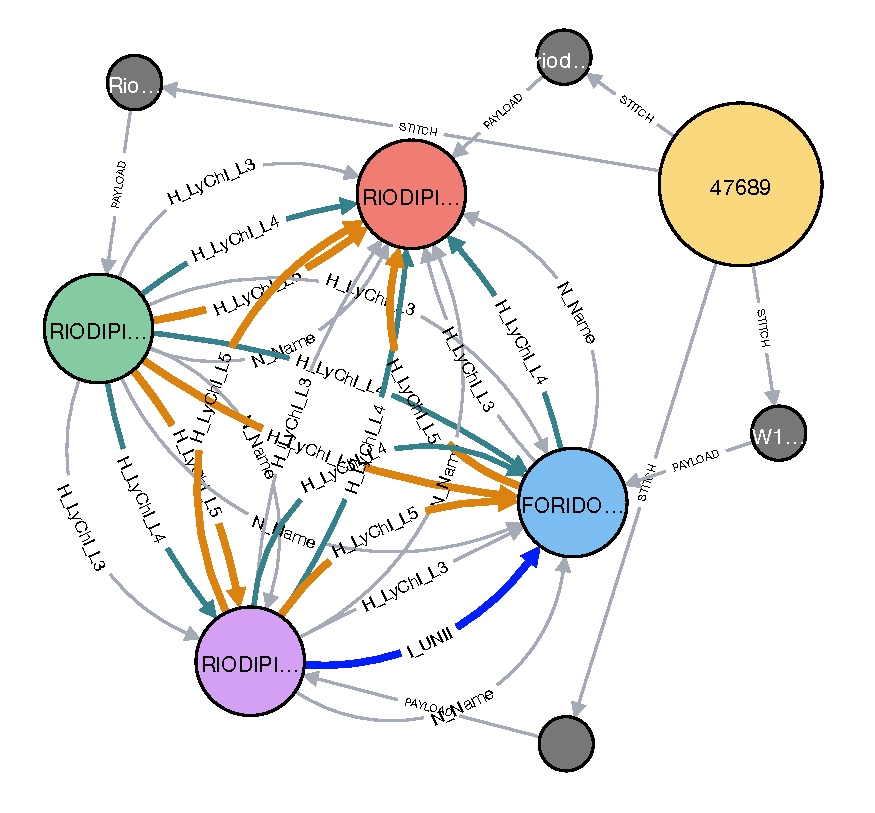
\includegraphics[scale=0.5]{graph3}}
\end{figure}

\begin{figure}[!ht]
  \caption{Chemical structures for (a) acetylsalicylic acid and (b) ethyl
    acetylsalicylate.}\label{fig:aspirin} 
  \centerline{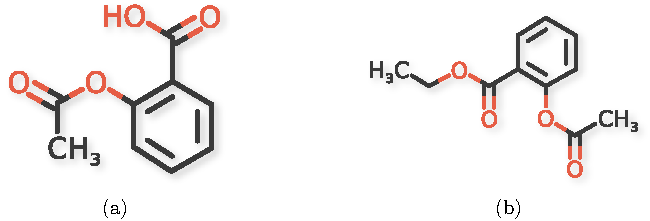
\includegraphics[scale=0.7]{aspirin-fig-crop}}
\end{figure}

\begin{figure}[ht!]
  \caption{A connected component for ASPIRIN.}\label{fig:ASPIRIN}
  \centerline{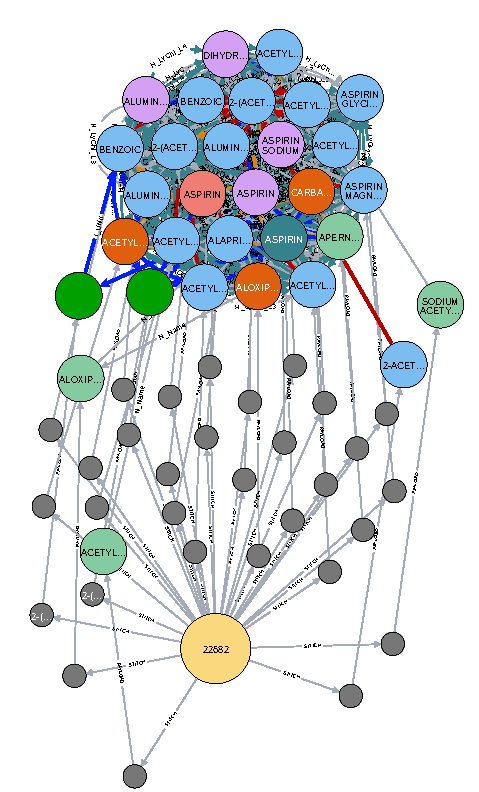
\includegraphics[scale=0.5]{graph5-crop}}
\end{figure}

\begin{figure}[ht!]
  \caption{A connected component for LEVOMETHADYL that clearly shows two
    distinct clusters.}\label{fig:LEVOMETHADYL}  
  \centerline{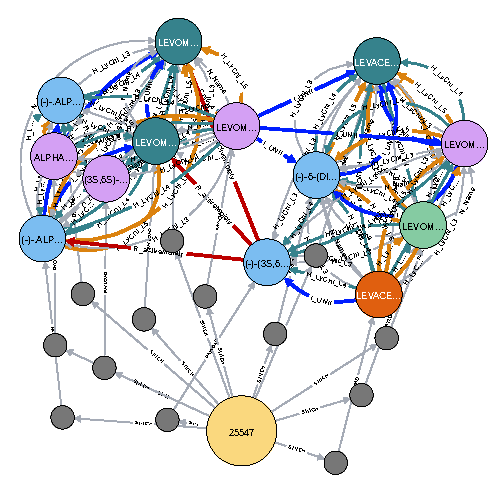
\includegraphics[scale=0.5]{graph6-crop}}
\end{figure}

\begin{figure}[ht!]
  \caption{A dense connected component for BENOXAPROFEN that resolved to
    three unique entities.}\label{fig:BENOXAPROFEN}
  \centerline{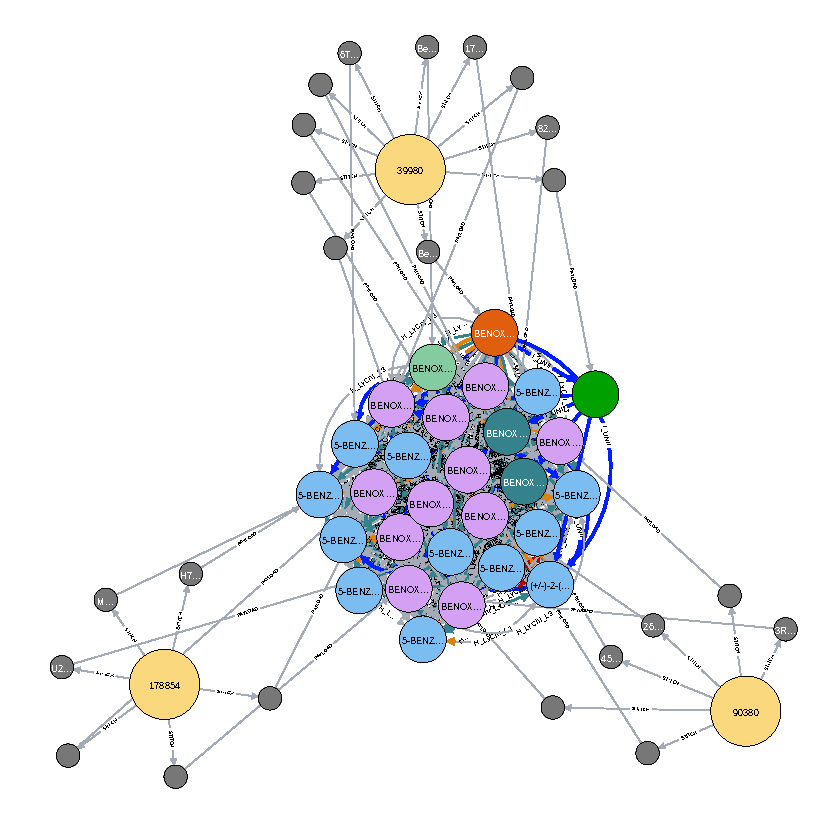
\includegraphics[scale=0.5]{graph4-crop}}
\end{figure}

%%%%%%%%%%%%%%%%%%%%%%%%%%%%%%%%%%%
%%                               %%
%% Tables                        %%
%%                               %%
%%%%%%%%%%%%%%%%%%%%%%%%%%%%%%%%%%%

%% Use of \listoftables is discouraged.
%%
\section*{Tables}

\begin{table}[ht!]
  \caption{An example of integrating data from multiple
    sources where each source contains only partial
    information.\label{tab:data-integration-example}}
  \begin{tabular}{ccllll}\toprule
    Source& ID & Name & CAS & UNII & Structure\\ \midrule
    A & 1 & \vtop{\hbox{ESOMEPRAZOLE}\vspace{2pt}
      \hbox{STRONTIUM}\vspace{2pt}\hbox{ANHYDROUS}\vspace{2pt}} & 914613-86-8 &
    \texttt{SCC2RK476A} & Correct\\
    A& 2 & ESOMEPRAZOLE & 217087-09-7 & \texttt{N3PA6559FT} & Correct\\
    A& 3 & OMEPRAZOLE & 95382-33-5 & \texttt{KG60484QX9} & Correct\\
    A& 4 & \vtop{\hbox{OMEPRAZOLE}\vspace{2pt}\hbox{SODIUM}} &
    95510-70-6 & \texttt{KV03YZ6QLW} & Correct\\ 
    B& 1 & Esomeprazole & & \texttt{C5N25H3803} & Correct\\
    B& 2 & Omeprazole & & \texttt{KV03YZ6QLW} & Correct\\
    C& 1 & OMEPRAZOLE, (R)- & 119141-89-8 & \texttt{S51HU491WJ} & Correct\\
    C& 2 & OMEPRAZOLE & 73590-58-6 & \texttt{KG60484QX9}& Correct\\
    C& 3 & ESOMEPRAZOLE & 119141-88-7 & \texttt{N3PA6559FT} & Correct\\
    D& 1 & esomeprazole & 161973-10-0 & & Correct\\
    D& 2 & omeprazole &
    \vtop{\hbox{73590-58-6}\vspace{2pt}
      \hbox{95510-70-6}\vspace{2pt}
      \hbox{95382-33-5}\vspace{2pt}
      \hbox{131959-78-9}\vspace{2pt}
      \hbox{172964-80-6}\vspace{2pt}
      \hbox{161796-78-7}\vspace{2pt}} & & Incorrect\\
    D& 3 & esomeprazole & & & None\\
    E& 1 & Omeprazole & 73590-58-6 & & None\\ \bottomrule
  \end{tabular}
\end{table}

\begin{table}[ht!]
\caption{Stitch keys and stitch values for the
drug \emph{imatinib mesylate}.\label{tab:imatinib}}
\begin{tabular}{@{}ll@{}}\toprule
  Stitch key & Stitch value\\ \midrule
\texttt{N\_Name} & \texttt{IMATINIB MESYLATE}; \texttt{GLEEVEC}; \texttt{GLIVEC}\\
\texttt{I\_UNII} & \texttt{8A1O1M485B}\\
\texttt{I\_CAS} & \texttt{220127-57-1}\\
\texttt{I\_CID} & \texttt{5291}\\
\texttt{I\_CODE} & \texttt{STI-571}; \texttt{CHEMBL941}\\
\texttt{H\_LYCHI\_L5} & \texttt{7S4GKGNQ6N3X-N}\\
\texttt{H\_LYCHI\_L4} & \texttt{VLU17BQBSGWU-N}; \texttt{K83X3L3XSSHK-S}\\
\texttt{H\_LYCHI\_L3} & \texttt{VL3FPUQ59CU-N}; \texttt{K846NBMB7T3-S}\\
\texttt{R\_activeMoiety} & \texttt{BKJ8M8G5HI}\\ \bottomrule
\end{tabular}
\end{table}

\begin{table}[ht!]
\caption{Distribution of edge types for the stitch multigraph.\label{tab:stitch-keys}}
\begin{tabular}{@{}ll@{}}\toprule
Stitch key & Size\\ \midrule
\texttt{H\_LyChI\_L3}	& 6,140,942\\
\texttt{H\_LyChI\_L4} &	5,300,078\\
\texttt{N\_Name} &	177,446\\
\texttt{H\_LyChI\_L5} &	162,160\\
\texttt{I\_UNII} &	139,176\\
\texttt{R\_activeMoiety} & 14,940\\
\texttt{I\_CAS}	& 11,684\\
\texttt{I\_CID} &	2,044\\ \bottomrule
\end{tabular}
\end{table}

\begin{table}[ht!]
\caption{Top stitch values for each stitch key. The LyChI hash keys
  \texttt{L3} and \texttt{L4} correspond to the potassium ion
  (K$^+$).\label{tab:stitch-values}}
\begin{tabular}{@{}lll@{}}\toprule
Stitch key & Stitch value & Size\\ \midrule
\texttt{H\_LyChI\_L3}	& \texttt{VUSPQLGXN18-M} &	1,344,440\\
\texttt{H\_LyChI\_L4} &	\texttt{VU8BQZFPPYTZ-M} & 1,307,592\\
\texttt{N\_Name} & \texttt{ROFECOXIB} &72 \\
\texttt{H\_LyChI\_L5} &	\texttt{9DKQLD7D29DN-N} & 162,160\\
\texttt{I\_UNII} & \texttt{UNKNOWN} &210 \\
\texttt{R\_activeMoiety} & \texttt{2M83C4R6ZB} & 106\\
\texttt{I\_CAS}	& \texttt{25322-68-3} & 1,806\\
\texttt{I\_CID} & \texttt{121225712} & 380\\ \bottomrule
\end{tabular}
\end{table}

\begin{table}[ht!]
\caption{Data sources used in the current version of \st.\label{tab:data-sources}}
\begin{tabular}{@{}ll@{}}\toprule
Data source & Size\\ \midrule
G-SRS, April 2019&	105,019\\
Withdrawn and Shortage Drugs List Feb 2018 &	674\\
Broad Institute Drug List 2018-09-07 &	6,125\\
NCATS Pharmaceutical Collection, April 2012 &	14,814\\
Rancho BioSciences, March 2019 &	51,591\\
Pharmaceutical Manufacturing Encyclopedia (Third Edition) &	2,268\\
DailyMed Rx, July 2020 &	74,850\\
DrugBank, July 2020&	11,922\\
DailyMed Other, July 2020&	13,393\\
DailyMed OTC, July 2020&	79,448\\
Drugs\@FDA \& Orange Book, July 2019&	28,256\\
ClinicalTrials, December 2017&	305,833\\
OTC Monographs, December 2018&	2,713\\
FDA NADA and ANADAs, December 2018&	554\\
FDA Excipients, December 2018&	10,212\\ \bottomrule
\end{tabular}
\end{table}

\section*{Algorithms}
\begin{algorithm}[ht!]\label{algo:stitching}
\SetKwInOut{Input}{Input}
\SetKwInOut{Output}{Output}
\SetKwFunction{Union}{Union}
\SetKwFunction{Find}{Find}
\SetAlgoLined
\DontPrintSemicolon
Let $W$ denote the set of stitch nodes created in the data ingestion
step for a given data source $D$.\\
Let $\langle k, v\rangle$ be the tuple of stitch key and value,
respectively, defined for a stitch node $w$.\\
$G=(V,E)$ is the current stitch multigraph.\\
\Find{$k, v$} is a function that returns all stitch nodes in $V$
containing stitch key $k$ and stitch value $v$.\\
\Union{$w,z$} is a union-find algorithm for tracking disjoint sets
(i.e., connected components).\\
 \For{$w \in W$}{
    \For{$\langle k_i, v_i\rangle \in w$}{
      \For{$z \in$ \Find{$k_i,v_i$}}{
         $E \leftarrow E \cup z\thicksim w$\;
         \Union{$w,z$}\;
      }
    }
    $V \leftarrow V \cup w$\;
 }
 \caption{Entity stitching algorithm}
\end{algorithm}

\begin{algorithm}[ht!]\label{algo:untangle}
\SetKwFunction{MergeNodes}{MergeNodes}
\SetKwFunction{MergeCliques}{MergeCliques}
\SetKwFunction{MergeSingletons}{MergeSingletons}
\SetAlgoLined
\DontPrintSemicolon
Let $U$ be the disjoint set data structure for all entities.\\
Let $S$ denote the set of unlabeled entities (i.e., singletons).\\
$C=(V,E)$ is the connected component.\\
\MergeNodes{$U, r$} is a function that performs transitive closure on
stitch nodes in $C$ which are connected by a relation $r\in E$. The results are
accumulated in $U$.\\
\MergeCliques{$U, K$} is a function that takes a set of stitch keys
$K$, finds overlapping cliques that span two or more stitch keys,
and performs transitive closure on the entities.\\
\MergeSingletons{$U, S, K$} is a function that also takes in a set of
stitch keys $K$, a set of singleton stitch node $S$, and find the best
mapping to an already labeled stitch node.\\
\MergeNodes{$U,$\texttt{R\_activeMoiety}}\;
\MergeNodes{$U,$\texttt{I\_UNII}}\;
\MergeNodes{$U,$\texttt{H\_LyChI\_L4}}\;
\MergeCliques{$U,$\texttt{N\_Name},\texttt{I\_CAS},\texttt{I\_CID},\texttt{H\_LyChI\_L4}}\;
\MergeSingletons{$U,S,$\texttt{N\_Name},\texttt{I\_CAS}}\;
 \caption{An algorithm to untangle a connected component}
\end{algorithm}

%%%%%%%%%%%%%%%%%%%%%%%%%%%%%%%%%%%
%%                               %%
%% Additional Files              %%
%%                               %%
%%%%%%%%%%%%%%%%%%%%%%%%%%%%%%%%%%%

%\section*{Additional Files}
%  \subsection*{Additional file 1 --- Sample additional file title}
%    Additional file descriptions text (including details of how to
%    view the file, if it is in a non-standard format or the file extension).  This might
%    refer to a multi-page table or a figure.
%
%  \subsection*{Additional file 2 --- Sample additional file title}
%    Additional file descriptions text.

\end{backmatter}
\end{document}
